\documentclass[10pt,letterpaper]{article}
\usepackage[anonymize=true]{cogsci}
\usepackage[style=apa,natbib=true,annotation=false]{biblatex}
\addbibresource{refs.bib}
\setlength{\bibhang}{.125in}
\usepackage{amsmath,graphicx,booktabs}
\newcommand{\RR}{\mathrm{RR}}
\newcommand{\ER}{\mathrm{ER}}
\title{Caution Adjusts Less Than the Reward-Rate Optimum Across Error Penalties}
\author[1]{\mbox{Author N. One}}
\affil[1]{Department, University}
\begin{document}
\maketitle
\begin{abstract}
Larger error penalties increase response caution, but this does not establish whether adjustment matches the reward-rate optimum. We analyzed a speeded choice task in which 358 participants faced five penalties from 5 to 80 points. Drift-diffusion thresholds increased at a median 38\% of the optimal slope, with overcaution at low penalties and undercaution at high penalties. Estimated reward rates nevertheless averaged 94\% of the conditional optimum. A policy penalizing departures from a fitted reference threshold predicted withheld penalty levels better than a subjective-penalty model. Its advantage over a descriptive rule depended on whether penalties could also affect drift and non-decision time. Memory load was associated with a higher reference threshold; allowing separate costs by load did not improve prediction. These results extend established incentive and control-cost accounts by quantifying graded miscalibration. They support a reference-based description of adjustment without identifying adjustment effort as its cause.

\textbf{Keywords:} speed--accuracy trade-off; decision threshold; error penalties; reward rate; cognitive control
\end{abstract}

\section{Introduction}
An error can be cheap in one setting and expensive in another. A decision maker who responds appropriately to this change should require more evidence when errors become costly. Yet a change in the right direction need not be large enough. Someone may become more cautious as penalties rise while moving progressively farther below the caution that maximizes expected points per unit time. The size of the adjustment, rather than its direction alone, is therefore central to evaluating adaptation to incentives.

The drift-diffusion model (DDM) provides a way to separate response caution from other sources of slow responding \citep{ratcliff1978,ratcliff2008}. Evidence accumulates at drift rate $v$ until it reaches a decision boundary. Increasing boundary separation $a$ generally improves accuracy but takes longer. Non-decision time $t_0$ captures processes outside evidence accumulation. Given these parameters and the time between responses, a reward-rate calculation specifies the threshold that maximizes expected earnings \citep{bogacz2006}. Holding the other quantities fixed, a larger error penalty favors a higher threshold.

Several components of this account are already supported by evidence. \citet{leng2021} varied rewards and punishments in a self-paced Stroop task and found that larger punishments increased DDM thresholds, consistent with their normative control model. Their experiments used two and three incentive levels. Thus, neither an effect of punishment on caution nor a reward-rate account of that effect is new here. Our question concerns how closely the magnitude of threshold adjustment follows a participant-specific, objective point-rate benchmark across five penalty levels.

Studies of reward-rate optimization also establish that people can choose thresholds above the estimated optimum \citep{bogacz2010,simen2009,starns2012}. This is not an invariant human preference: practice and guidance can bring performance closer to optimal policies \citep{balci2011,evans2017}. A further distinction concerns the consequences of a threshold error. A substantial deviation in threshold need not imply a substantial loss of reward. \citet{malhotra2017} demonstrated relatively inexpensive deviations in a task involving time-varying decision boundaries. That result motivates a separate assessment of the earnings associated with miscalibration, rather than treating distance from the optimum as a direct measure of performance loss.

Conservative adjustment also has precedents outside sequential sampling. Payoff-sensitive categorization studies show that response criteria can move less than prescribed by a decision-theoretic benchmark \citep{maddox1998}. A criterion separating response categories is different from a DDM boundary controlling how much evidence to collect. The conceptual resemblance is useful, but it neither establishes a common mechanism nor makes the two measures interchangeable.

The possibility that adjustment itself is costly is also established. Resource-rational accounts and the expected value of control framework evaluate control in relation to its benefits and costs \citep{lieder2020,shenhav2013}. More directly, \citet{grahek2022} found smaller within-task control adjustments when performance goals varied frequently, and modeled a cost on the distance between control configurations. Their account already links attenuated adjustment to control reconfiguration. We build on that proposal by evaluating a cost centered on a stable, load-specific reference threshold, and by comparing it with a threshold anchored to the previous block. The term \emph{reference} describes a fitted model parameter; it does not imply that we measured an initial or habitual threshold independently.

We test whether fitted thresholds track the magnitude of the optimal adjustment across five penalties and whether deviations change sign within that range. We then compare reference-based adjustment, subjective penalties, and a descriptive rule. The empirical contribution is the joint quantification of relative sensitivity and signed deviations; the modeling contribution is the comparison of reference-based policies. Established incentive effects, control-cost ideas, and near-optimal reward efficiency provide the foundation for this analysis.

\section{Method}
\subsection{Participants and Data}
The Suboptimality Task was part of a broader computerized cognitive battery. The available task dataset contained 365 participants. Preprocessing retained participants with accuracy at least .70, at least 85\% of responses between 0.2 and 3 s, and estimated per-trial overhead between 0.3 and 1.5 s in each load condition. Seven participants were excluded, leaving 358. Their records contained 191,839 trials, of which 190,506 fell inside the fitting window. Participants contributed about 536 recorded trials on average; the median block contained 46 trials. Cognitive ability composites were available for 277 included participants.

\subsection{Suboptimality Task}
Participants repeatedly performed a simple, speeded two-choice task within twelve 60-s blocks (Figure~\ref{fig:task}A). Each correct response earned 20 points, whereas each error lost $P\in\{5,10,20,40,80\}$ points. The penalty was fixed within a block. This design creates a trade-off: faster responding provides more opportunities to earn points, but errors become progressively more expensive as the penalty increases. The ratio of error loss to correct-response reward ranges from 0.25 to 4. The analysis asks whether participants adjust caution in proportion to the change in the optimal policy, rather than merely responding more slowly when penalties are high.

The penalty manipulation was crossed with a concurrent letter-memory requirement. In the load condition, participants retained letters while performing the choice task; the existing description places letter presentation during feedback. The no-load condition omitted this additional memory requirement. Each penalty appeared once per load, except 20 points, which appeared twice, yielding six blocks per load and twelve in total. Block order was randomized according to the existing task description. The schematic summarizes these manipulations without reconstructing the unspecified stimulus display. Exact choice stimuli, response mapping, letter-set size, memory test, recruitment, compensation, ethics approval, and the source citation remain to be verified against the collection protocol.

\begin{figure}[t]
\centering
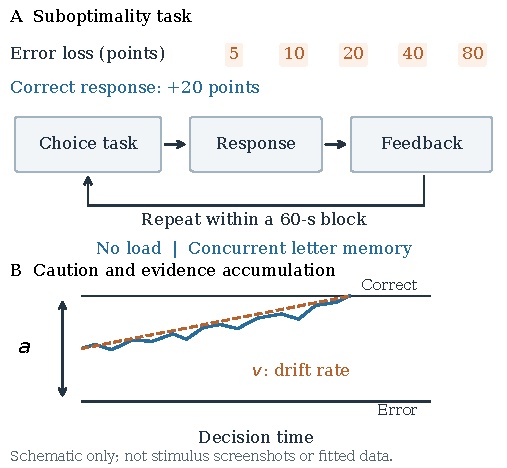
\includegraphics[width=\columnwidth]{figs/fig0_task.pdf}
\caption{Task and model overview. (A) Speeded choices repeat within a fixed time budget, with a constant reward, varying error penalties, and two memory-load conditions. (B) An illustrative accuracy-coded DDM trajectory starts halfway between the boundaries. Separation $a$ indexes caution; drift $v$ indexes evidence accumulation. The diagram is conceptual, not an experimental screenshot or a fitted trajectory.}
\label{fig:task}
\end{figure}

\subsection{Cognitive Ability Measures}
The battery assessed four related abilities. Working memory capacity (WMC) concerns maintaining information while processing other material and was assessed with Operation Span, Symmetry Span, and Rotation Span. Fluid intelligence (gF) concerns reasoning about relations and patterns and was assessed with Raven's Advanced Progressive Matrices, Number Series, and Letter Sets. Attention control (AC) concerns selecting goal-relevant information; the task notes list Squared Simon, Visual Array, and Antisaccade. Sustained attention concerns maintaining task engagement over time; its measures included the Sustained Attention to Response Task, Sustained Attention-to-Cue Task, and Psychomotor Vigilance Task.

We analyzed the supplied WMC, gF, AC, and sustained-attention (SuS\_AC) composites, rather than treating each task score as an independent test. The exact composite scoring and the AC task subset require source confirmation: the score file also contains other conflict tasks. These between-person measures are distinct from the within-person letter-memory manipulation. A load effect therefore tests a change in task demands, whereas a composite association describes differences among participants.

\subsection{Estimating Caution and Its Benchmark}
We fit an accuracy-coded DDM with starting point $a/2$ and diffusion coefficient fixed at 1. The likelihood used the first-passage density described by \citet{navarro2009}, mixed with a 2\% contaminant distributed uniformly over response type and the 0.2--3-s window. Fits excluded responses outside this window. In the primary parameterization, $v$ and $t_0$ differed between load conditions but were shared across penalties. A model with ten separately fitted thresholds, one per penalty and load combination, provided the empirical estimates used to characterize adjustment. These thresholds are inferred from behavior; they are not directly observed or constrained to follow the reference-cost policy.

For boundary separation $a$ and positive drift $v$, the model gives
\begin{equation}
\ER(a)=\frac{1}{1+e^{va}},\qquad
\mathrm{DT}(a)=\frac{a}{2v}\tanh\!\left(\frac{va}{2}\right).
\end{equation}
The expected net point rate is
\begin{equation}
\RR(a;P)=\frac{20[1-\ER(a)]-P\ER(a)}{\mathrm{DT}(a)+t_0+T}.
\label{eq:rr}
\end{equation}
We estimated overhead in each block as $(60-\sum\mathrm{RT})/n$, then took its median within participant and load. Median overhead across included participants was 0.537 s without load and 0.567 s with load. This estimate absorbs feedback, inter-trial time, and any unused end-of-block time. It is an inferred timing quantity, not a direct measurement of stimulus durations.

For each participant and load, $a^*(P)=\arg\max_a\RR(a;P)$ was calculated on a grid from 0.05 to 5.0, with local parabolic refinement. We call this the \emph{conditional optimum}: drift, non-decision time, and overhead are held at their fitted or estimated values. It is not an optimum over all possible changes to attention, memory, or task strategy. Equation~\ref{eq:rr} is a stationary reward-rate benchmark for the fixed-duration task, rather than an exact solution to the finite-horizon problem near the end of a block.

\subsection{Quantifying Adjustment and Efficiency}
Within each participant and load, we regressed the five estimated thresholds on $x=\log_2(P/20)$ and calculated the corresponding slope for the five optimal thresholds. We averaged the slopes over load, then divided the fitted slope by the optimal slope. A ratio of 1 indicates matched linear sensitivity over this penalty range; a ratio of 0 indicates no linear adjustment. The ratio summarizes a five-point function and should not be interpreted as a constant fraction of the optimum at every penalty. Group estimates report the median of participant ratios, not the ratio of group-average slopes.

We assessed overcaution and undercaution separately using $a(P)-a^*(P)$. A flatter function does not by itself imply that this difference changes sign. To test the crossover directly, we averaged thresholds over load within participant, then computed the signed difference at each endpoint. We also counted participants whose estimated difference was positive at 5 points and negative at 80 points. For efficiency, we computed $\RR(a;P)/\RR(a^*;P)$ in each condition and averaged across conditions and participants. This is an estimated expected-rate ratio, not observed points divided by an empirically attainable score.

\subsection{Candidate Threshold Policies}
Each policy maps the displayed penalty to a threshold while retaining four DDM parameters, $v$ and $t_0$ for each load. The main reference-cost policy adds two reference thresholds and one shared positive cost:
\begin{equation}
\hat a(P,\ell)=\arg\max_a\{\RR(a;P,\ell)-c(a-a_0^\ell)^2\}.
\label{eq:cost}
\end{equation}
Here $\ell$ denotes load, $a_0^\ell$ is the reference, and $c$ controls the penalty for departing from it. The objective uses points per second, without normalization by the optimal reward rate. Consequently, the numerical scale of $c$ depends on the units of reward and threshold. This seven-parameter policy is a computational hypothesis about the shape of adjustment, not a direct measurement of experienced effort.

We compared three eight-parameter alternatives. A separate-cost policy permits a different $c$ for each load. A subjective-penalty policy substitutes $\lambda_\ell20(P/20)^{\gamma_\ell}$ for $P$ when calculating the optimal threshold; values $\gamma_\ell<1$ compress the penalty range. A log-linear policy sets $\ln a=\alpha_\ell+\beta_\ell\log_2(P/20)$ without a reward-rate objective. A further sequential comparison replaces the fixed reference with the previous block's predicted threshold, using the load-specific reference for the first block. This implements one previous-state alternative inspired by reconfiguration-cost models, not a reproduction of the full drift-and-threshold model of \citet{grahek2022}.

\subsection{Prediction, Uncertainty, and Robustness}
The existing analysis used five leave-one-penalty-out folds per participant. Each fit used trials from four penalties in both load conditions; the likelihood of responses at the fifth penalty provided the evaluation score. Holding out an endpoint tests extrapolation over the sampled range, whereas holding out an interior value tests interpolation. We compare summed log likelihoods and participant-level wins. We also report threshold prediction errors, because a likelihood difference need not translate into a large difference in threshold accuracy.

The implementation has a qualification: fits used an initialization from the full dataset, $t_0$ bounds based on the full-data minimum response time, and overhead estimated from all blocks. These procedures share information with the withheld condition. We therefore describe the scores as withheld-penalty comparisons with shared preprocessing, not fully independent validation. A training-only rerun is needed before making strong claims about out-of-sample superiority. Withholding a penalty also does not test new participants, tasks, or samples.

Uncertainty summaries use 2,000 participant bootstrap resamples. Existing random split-half checks partitioned the same participants 1,000 times. These checks assess within-sample stability; they are not independent replications. For individual differences, hierarchical estimates used a Gaussian prior on transformed parameters with expectation--maximization and a Laplace approximation \citep{huys2011}. Partial Spearman correlations controlled for average drift and used Benjamini--Hochberg correction across 16 tests. Recovery simulations and expanded DDM parameterizations assessed whether conclusions depended on estimation noise or the assumption that penalties influence only thresholds.

\section{Results}
\subsection{Adjustment Was Shallower Than the Optimum}
Thresholds increased with the error penalty (Figure~\ref{fig:threshold}). Averaging over load within participant, median fitted thresholds increased from 1.51 at 5 points to 1.96 at 80 points. Corresponding median optima increased from 1.05 to 2.16. The median relative slope was 0.382, with a bootstrap 95\% confidence interval (CI) of [0.313, 0.448]. In 88\% of participants, the fitted slope was below the optimal slope. Thus, the central result is a substantial attenuation relative to a defined normative benchmark, not simply a positive punishment effect.

Signed deviations support a crossover at the group level. The median within-participant difference $a-a^*$ was 0.466 at 5 points (95\% CI [0.430, 0.504]) and $-0.243$ at 80 points (95\% CI [$-0.324$, $-0.173$]). Both signs occurred in the same participant's fitted endpoint estimates for 66\% of the sample. The group crossover therefore does not imply that every participant crossed, and this percentage does not establish reliable individual crossovers after accounting for parameter uncertainty. It describes the fitted estimates.

Despite this mismatch, the mean modeled efficiency ratio was .939 (95\% CI [.932, .945]). The large reduction in adjustment sensitivity coexisted with a relatively small expected point-rate loss. This result supports the established distinction between parameter optimality and reward efficiency. It does not establish that participants explicitly accepted a particular reward loss or optimized a subjective effort objective.

\begin{figure}[t]
\centering
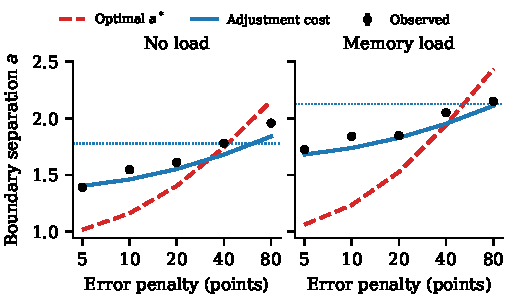
\includegraphics[width=\columnwidth]{figs/fig1_threshold.pdf}
\caption{Estimated caution across penalties. Points show means of separately fitted DDM thresholds with SEM; they are model estimates, not raw observations. Dashed curves show mean conditional optima. Solid curves show the reference-cost policy, and dotted lines its mean fitted reference. Text summaries use participant medians.}
\label{fig:threshold}
\end{figure}

\subsection{Reference-Cost Fits Compared Favorably}
Withheld-penalty log likelihoods favored the shared-cost policy among the four primary candidates (Table~\ref{tab:cv}). Its advantage over subjective penalties was 928 (95\% CI [423, 1,415]), and its advantage over the log-linear policy was 2,421 (95\% CI [1,845, 3,048]). These are aggregate comparisons under the shared-preprocessing procedure described above. The shared-cost policy was best for 190 of 358 participants and beat subjective penalties for 65\%. Group preference should not be read as a universal participant strategy.

\begin{table}[t]
\centering
\caption{Primary withheld-penalty comparison. Larger log likelihood is better. Counts include DDM parameters.}
\label{tab:cv}
\begin{tabular}{lrr}
\toprule
Policy & Parameters & Log likelihood\\
\midrule
Shared reference cost & 7 & $-46{,}737$\\
Separate costs by load & 8 & $-47{,}302$\\
Subjective penalties & 8 & $-47{,}665$\\
Log-linear threshold & 8 & $-49{,}158$\\
\bottomrule
\end{tabular}
\end{table}

The advantage was largest when an endpoint penalty was withheld (Figure~\ref{fig:cv}). However, mean absolute threshold errors were similar: 0.26 for reference cost, 0.26 for subjective penalties, and 0.28 for the log-linear policy. The difference in mean error between subjective penalties and reference cost was .0038 (95\% CI [$-.0040$, .0123]). The likelihood advantage therefore supplies evidence about predicted response distributions, with little evidence for a corresponding overall improvement in threshold error.

The fixed-reference implementation also exceeded the previous-block implementation by 3,793 log-likelihood units (95\% CI [2,628, 5,016]). This comparison favors a stable reference within the tested policy family and task. It does not rule out history dependence with other timescales, learned references, or changes in both drift and threshold.

\begin{figure}[t]
\centering
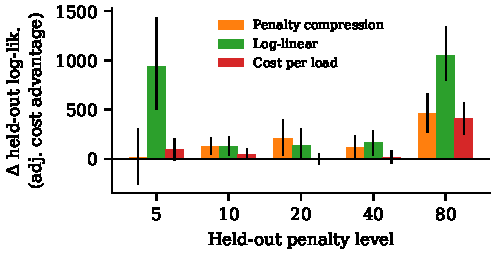
\includegraphics[width=\columnwidth]{figs/fig2_cv.pdf}
\caption{Summed withheld-penalty log-likelihood differences favoring reference cost, with participant-bootstrap 95\% CIs. Positive values favor the shared reference-cost policy. These comparisons inherit full-data initialization, bounds, and overhead estimates.}
\label{fig:cv}
\end{figure}

\subsection{What the Reference Cost Implies}
The policy supplies a simple explanation of how deviations can change sign. Let $a^*$ maximize a reward function $f$, and let $\hat a$ maximize $f(a)-c(a-a_0)^2$ over the same admissible set, with $c>0$. Comparing these two solutions gives
\begin{align}
f(\hat a)-c(\hat a-a_0)^2 &\geq f(a^*)-c(a^*-a_0)^2,\nonumber\\
f(a^*)&\geq f(\hat a).
\end{align}
Adding and dividing by $c$ yields
\begin{equation}
|\hat a-a_0|\leq |a^*-a_0|.
\label{eq:distance}
\end{equation}
This distance result alone does not establish which side of the optimum the choice occupies. If $f$ is unimodal with peak $a^*$ and both $a_0$ and $a^*$ are admissible, a stronger statement follows: $\hat a$ lies between them. Outside that interval, moving toward it weakly improves reward and strictly reduces the quadratic penalty. The choice is therefore at or above the optimum when $a^*\leq a_0$, and at or below it when $a^*\geq a_0$.

A crossover across penalties consequently requires the optimum to pass the reference within the tested range. It is not guaranteed for every reference or reward function. The inequalities are weak; strict deviations require further conditions. The existing Lean files formalize the distance and between-results under explicit hypotheses. These are mathematical properties of the policy, not evidence that people incur a literal effort cost. They also do not guarantee the empirical value .38, or a smaller derivative at every penalty. The quantitative slope result comes from the fitted data.

A local approximation clarifies the role of the reward landscape. Suppose that, near an interior optimum, reward is approximately $f(a^*)-\kappa(a-a^*)^2/2$, with curvature $\kappa>0$. Maximizing this approximation minus the reference cost gives
\begin{equation}
\hat a\ \approx\ \frac{\kappa}{\kappa+2c}a^*+
\frac{2c}{\kappa+2c}a_0.
\label{eq:local}
\end{equation}
For a fixed curvature, the solution is a weighted average of the optimum and reference. Larger cost increases attraction to the reference; a steeper reward surface increases attraction to the optimum. This derivation explains why adjustment and earnings should be assessed separately. A shallow surface makes departures from the optimum relatively inexpensive and permits a modest cost to have a sizable effect on the chosen threshold. However, curvature can vary with the penalty. The weight in Equation~\ref{eq:local} is therefore not necessarily constant, and the observed slope ratio cannot simply be inverted to recover an effort cost. This approximation explains the policy rather than introducing another fitted result.

\subsection{Memory Load and Individual Differences}
Memory load was associated with greater caution and a higher fitted reference (Figure~\ref{fig:load}A). Median references were 1.60 without load and 1.93 with load; 78\% of participants had an increase. The mean paired shift was .353 (95\% CI [.278, .423]). Hierarchical estimates gave similar medians, 1.63 and 1.97. Allowing a separate cost by load reduced withheld-penalty log likelihood by 565 (95\% CI for the shared-cost advantage [308, 825]). Thus, a reference shift with a shared cost was sufficient in this comparison. This is not an equivalence test demonstrating that load has no effect on cost or on penalty sensitivity.

In the 277 participants with composites, larger estimated cost was associated with lower sustained attention (partial $r_s=-.216$, $q=.0025$). A higher no-load reference was associated with lower attention control ($r_s=-.215$, $q=.0025$) and lower WMC ($r_s=-.207$, $q=.0028$). The load reference also correlated with WMC ($r_s=-.155$, $q=.031$). The load-related reference shift had no association surviving correction. These associations are exploratory and concern fitted parameters, not independently measured effort costs.

\begin{figure}[t]
\centering
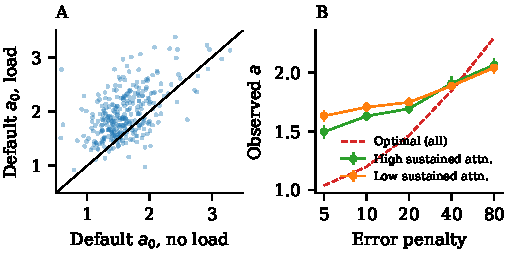
\includegraphics[width=\columnwidth]{figs/fig3_load_inddiff.pdf}
\caption{(A) Fitted reference thresholds by load, with the identity line. (B) Mean fitted thresholds for upper and lower sustained-attention quartiles, with SEM. The dashed optimum is for the entire sample, not a matched optimum for either quartile; normative subgroup comparisons use participant-specific benchmarks.}
\label{fig:load}
\end{figure}

The sustained-attention quartiles showed the same direction of difference: the lower quartile had larger median $\ln c$ (2.26 versus 0.82, $q=.001$) and a lower relative slope (0.26 versus 0.52, $q=.005$). Continuous associations provide the more direct individual-difference evidence; quartiles are descriptive follow-ups, not additional replications. An association between greater cost and higher WMC ($r_s=.167$, $q=.022$) further cautions against interpreting $c$ as a single measure of cognitive limitation.

\subsection{Sensitivity to Modeling Assumptions}
Penalty manipulations need not selectively affect caution \citep{rae2014,voss2004}. In fits with separate $v$, $t_0$, and $a$ for each condition, each doubling of the penalty was associated with a median 3\% increase in drift and an 11-ms increase in $t_0$. BIC favored the larger model for 21\% of participants. Under this parameterization, the median relative threshold slope was .21 and 90\% of participants remained below the optimal slope. Attenuation was therefore not confined to the primary selective-influence assumption.

Policy ranking was more sensitive. When every policy allowed drift and non-decision time to vary linearly with log penalty, reference cost exceeded subjective penalties by 9,318 withheld log-likelihood units but fell below the log-linear policy by 1,010. The more flexible comparison does not support general superiority over a descriptive threshold rule. It also prevents an inference from the primary ranking to a uniquely identified adjustment-cost mechanism.

Recovery simulations generated sessions from each participant's reference-cost and subjective-penalty fits. At the aggregate level, the generating policy exceeded the other by 561 and 1,080 log-likelihood units, respectively. At the individual level, the generating policy was best among the tested alternatives for 66\% of cost-generated sessions and 35\% of subjective-penalty sessions. Recovery was therefore more informative about aggregate comparisons than individual classification. In cost-generated data, correlations between generating and recovered parameters were .92--.94 for drift, .76--.78 for references, and .70 for $\ln c$. Simulation recovery is conditional on these generating models and does not establish that either generated the human data.

\section{Discussion}
The main empirical result is a mismatch in the magnitude of adaptation. Participants increased caution with penalties, but their median sensitivity was about 38\% of the sensitivity prescribed by a conditional reward-rate benchmark. Signed endpoint comparisons showed excess caution at low penalties and insufficient caution at high penalties. This combination matters because a description based only on average overcaution would miss the direction change within the same incentive range.

The contribution extends established punishment effects \citep{leng2021}, deviations from reward-rate optimality \citep{bogacz2010,evans2017}, and reconfiguration-cost accounts \citep{grahek2022}. It combines a five-level, participant-specific comparison with the optimum and an evaluation of fixed-reference and previous-state policies. This is a specific extension of prior work, not a claim to discover incentive-sensitive caution or costly control adjustment.

Two features distinguish this assessment from reporting a main effect of incentives. First, the benchmark is personalized. The same threshold can be excessive for one participant and insufficient for another because drift and timing alter the reward landscape. A common group threshold would obscure that difference. Second, the sign of the deviation is evaluated at both ends of the range. An overall average near zero could conceal opposing errors, while a shallow slope could coexist with overcaution throughout the range. The endpoint analysis addresses the latter ambiguity directly. Its uncertainty intervals reflect resampling participants with their saved estimates, however, and do not propagate the full uncertainty of the fitted thresholds and optima. A joint estimation procedure would provide a stronger assessment of individual crossover probabilities.

The reference-cost policy provides a compact way to link the empirical patterns. When the reference falls above the optimum, it favors excess caution; when it falls below the optimum, it favors insufficient caution. The same rule can therefore describe apparently opposite departures without introducing separate preferences at low and high penalties. Its mathematical appeal is explanatory economy under stated assumptions. It is not a demonstration that a quadratic psychological cost exists, or that reference attraction is the only source of the crossover.

The high efficiency ratio is supporting evidence rather than a distinct novelty claim. Consistent with work on robust but imperfect boundaries \citep{malhotra2017}, appreciable threshold errors can be inexpensive in reward terms. Conversely, a small reward loss does not establish optimality under hidden costs. Many policies can perform similarly when the reward surface is shallow. This makes the predictive comparison useful, but also explains why comparable threshold errors and changes in ranking under alternative DDM assumptions deserve weight.

Policy comparisons are conditional on the candidate set. The subjective-penalty model tests one parametric distortion with reward held fixed; its poorer score does not reject other utility functions or inaccurate beliefs about task difficulty. The log-linear rule can describe systematic adjustment without an explicit cost. Its advantage when other DDM processes vary shows that a successful threshold description need not identify a unique psychological objective.

The load results similarly require a limited interpretation. A higher reference captured the change in caution economically within the fitted family. Related work on prospective memory links concurrent intentions to more conservative decisions \citep{heathcote2015}, but prospective remembering is not the same manipulation as retaining letters. Here, memory demands were also coupled to feedback content. Without a matched display control and direct manipulation of the hypothesized adjustment cost, the results cannot isolate the cognitive process responsible for the reference shift.

Several further limitations bear on mechanism. The benchmark fixes drift and non-decision time even though participants may jointly adapt multiple processes. Its overhead estimate comes from observed responses and does not independently validate task timing. The fitting window and contaminant model approximate the response distribution, and finite block endings may favor policies that differ from a stationary optimum. The parameter $a_0$ is estimated from the same task as adjustment, so it may summarize a stable preference, prior, habit, or measurement regularization. Additional candidates, including criterion variability and learning-sensitive policies \citep{benjamin2009,masis2023}, remain untested here. The current subjective-penalty comparison cannot exclude all forms of subjective utility.

The clearest next test would independently manipulate the reference and the frequency of incentive changes. Reference-based adjustment predicts that shifting a learned reference should shift the penalty at which deviations change sign. A previous-state account instead predicts systematic dependence on the immediately preceding setting. Re-estimating preprocessing within training folds and evaluating a new sample would strengthen the predictive comparison. Together with complete task documentation, these steps are needed before advancing the descriptive result into a causal account of adjustment effort.

The results establish graded under-adjustment and a group crossover relative to the conditional optimum, with reference cost providing a plausible computational account.

\clearpage
\section{Declaration of Generative AI Use}
Claude Code (Anthropic) was used to assist with experimental implementation and data analysis, while Codex (OpenAI) was used for minor writing and editing assistance. All research ideas, experimental designs, and scientific interpretations were developed by the authors, who take full responsibility for the final manuscript.

\printbibliography
\end{document}
